\section{Results}

%     maybe misclassifications of each model and show each index and highlight where the model focuses.
%     31/41/82/.../679 m1 m2 m3 actual
%     A  F  P /.../ G  +  -  +  +
%     negative emphasized there.
\subsection{Preliminary Results}

The feature selection algorithm for the baseline model found six sites that best discriminate the susceptibility of the training sequences (Table 3.1). Each position has specific set of amino acids that increase likelihood of a sequence being immune.

\begin{table}[ht]
  \centering
  \begin{tabular}[t]{ c | l }
    \hline
    \textbf{Pos} & \textbf{Acids that impede susceptibility} \\
    \hline
    83 & Phenylalanine (F) \\
    211 & Aspartate (D) \\
    212 & Alanine (A), Aspartate (D), Serine (S) \\
    246 & Arginine (R) \\
    251 & Valine (V) \\
    687 & Not Alanine (A) or Serine (S) \\
    \hline
  \end{tabular}
  \figcaption{Table}{Summary of feature selection algorithm results}
\end{table}

The eliminative algorithm based on the original study identified eight mutations that only appeared in immune sequences, shown in Table 3.2.

\begin{table}[ht]
  \centering
  \begin{tabular}[t]{ c | c  c  c }
    \hline
    \textbf{Pos} & \multicolumn{3}{c}{\textbf{Mutation}} \\
    \hline
    31 & Lysine (K) & $\to$ & Aspartate (D){\rule{0pt}{2.6ex}} \\[1mm]
    41 & Tyrosine (Y) & $\to$ & Alanine (A) \\[1mm]
    \multirow{2}{*}{66} & Glycine (G) & \multirow{2}{*}{$\Rightarrow$} & \multirow{2}{*}{Alanine (A)} \\
    & Arginine (R) \\[1mm]
    83 & Tyrosine (Y) & $\to$ & Phenylalanine (F) \\[1mm]
    \multirow{2}{*}{113} & Serine (S) & \multirow{2}{*}{$\Rightarrow$} & \multirow{2}{*}{Asparagine (N)} \\
    & Arginine (R) \\[1mm]
    353 & Lysine (K) & $\to$ & Histidine (H) \\[1mm]
    426 & Proline (P) & $\to$ & Serine (S) \\[1mm]
    679 & Isoleucine (I) & $\to$ & Valine (V) \\[1mm]
    \hline
  \end{tabular}
  \figcaption{Table}{Mutations that may abolish susceptibility (eliminative)}
\end{table}

\subsection{Structural Analysis}

By complementing the findings of the preliminary findings with a structural analysis, the feature set used for the structural model was reduced to five sites. 

\begin{figure}[ht!]
    \centering
    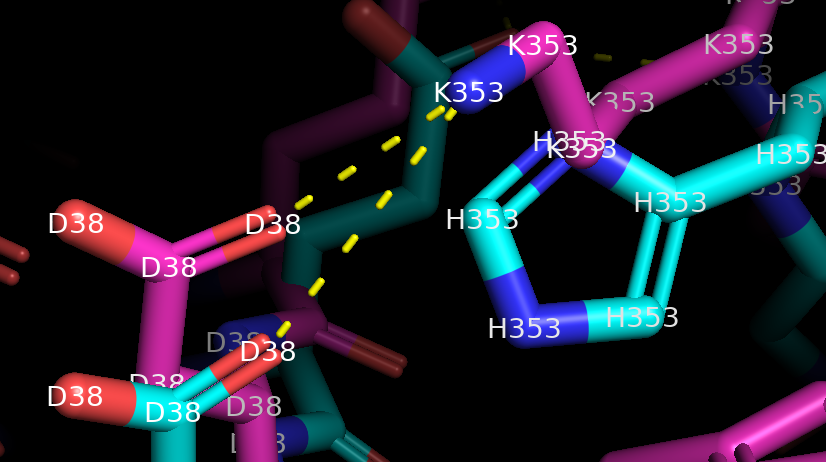
\includegraphics[width=\textwidth]{figures/structure-353.png}
    \figcaption{Figure}{The structural effect of mutation H353}
\end{figure}

As an sample of the findings of the investigation, Figure 3.1 depicts the change caused by the mutation at position 353 from lysine (K) to histidine (H). The human ortholog is coloured pink, and the rat ortholog containing the mutation is coloured cyan. This mutation abolishes a polar bond between the residue at position 353 and the aspartate (D) at position 38. Further, the lysine at position 353 in the human sequence displayed potential to bond with the virus spike protein, suggesting it may be a binding site. Since the mutation had an affect on the structure of the protein and there is evidence it may be a binding site, the mutation was included in the structural model. 

\begin{table}[ht]
  \centering
  \begin{tabular}[t]{ c | c  c  c }
    \hline
    \textbf{Pos} & \multicolumn{3}{c}{\textbf{Mutation}} \\
    \hline
    31 & Lysine (K) & $\to$ & Aspartate (D){\rule{0pt}{2.6ex}} \\[1mm]
    83 & Tyrosine (Y) & $\to$ & Phenylalanine (F) \\[1mm]
    \multirow{2}{*}{113} & Serine (S) & \multirow{2}{*}{$\Rightarrow$} & \multirow{2}{*}{Asparagine (N)} \\
    & Arginine (R) \\[1mm]
    353 & Lysine (K) & $\to$ & Histidine (H) \\[1mm]
    426 & Proline (P) & $\to$ & Serine (S) \\[1mm]
    \hline
  \end{tabular}
  \figcaption{Table}{Mutations that may abolish susceptibility (structural)}
\end{table}

The list of mutations used for the structural model is depicted in Table 3.3, and a more detailed overview of the structural analysis involved is included in Appendix B.

\subsection{Model Design}

With the set of mutations that abolish susceptibility identified for each model, three categorical binary decision trees were made for classification. Table 3.4 outlines the subset of positions selected for use in each model.

\begin{table}[ht]
  \centering
  \begin{tabular}[t]{ c | c  c  c | c }
    \hline
    & \multicolumn{3}{c|}{Model} \\
    \textbf{Pos} & \textbf{B} & \textbf{E} & \textbf{S} & \textbf{UniProt} \\
    \hline
    31 & & \texttimes & \texttimes & \texttimes \\
    41 & & \texttimes & & \texttimes \\
    66 & & \texttimes & & \\
    83 & \texttimes & \texttimes & \texttimes & \texttimes \\
    113 & & \texttimes & \texttimes & \\ 
    211 & \texttimes & & & \\
    212 & \texttimes & & & \\ 
    246 & \texttimes & & & \\
    251 & \texttimes & & & \\
    353 & & \texttimes & \texttimes & \texttimes \\
    426 & & \texttimes & \texttimes & \texttimes\\
    679 & & \texttimes & & \\
    687 & \texttimes & & & \\
    \hline
  \end{tabular}
  \figcaption{Table}{Positions of focus for each model}
\end{table}

Each marked cell indicates the position was used as a feature in the model of the column, where B, E, and S represent the baseline, eliminative, and structural models, respectively. The UniProt column is marked for each position where the UniProt database's mutagenesis overview identified the position as influential to susceptibility \cite{UniProt}. The UniProt database consolidates the findings of many studies to summarize how mutations affect susceptibility; this column represents a standard of comparison for the feature set of each model.

It is clear from this table that the structural model was most true to the findings outlined on UniProt, while the baseline model was not similar at all.

\subsection{Model Performance}

Each model was evaluated using its corresponding test set to produce confusion matrices (Table 3.5). The rows of the matrices represent the true class of the sequences, and the columns represent the model's predicted class.

\begin{table}[!htb]
    \figcaption{Table}{Classification confusion matrices for each model}
    \begin{subtable}{.33\linewidth}
      \centering
        \begin{tabular}{c|c|c}
            & + & -  \\
            \hline
            + & 5 & 1 \\
            - & 1 & 1 \\
        \end{tabular}
      \caption{Baseline Model}
    \end{subtable}%
    \begin{subtable}{.33\linewidth}
      \centering
        \begin{tabular}{c|c|c}
            & + & -  \\
            \hline
            + & 14 & 3 \\
            - & 3 & 6 \\
        \end{tabular}
      \caption{Eliminative Model}
    \end{subtable}%
        \begin{subtable}{.33\linewidth}
      \centering
        \begin{tabular}{c|c|c}
            & + & -  \\
            \hline
            + & 24 & 3 \\
            - & 5 & 9 \\
        \end{tabular}
      \caption{Structural Model}
    \end{subtable}%
\end{table}

The sensitivity (true positive rate), specificity (true negative rate), and accuracy for each model were computed based on the confusion matrices (Table 3.6). The structural model had the highest accuracy and sensitivity, meaning it was more successful than the other models at correctly identifying sequences that are susceptible, and more successful at classifying sequences overall \cite{Vu2015}. The eliminative model had a marginally higher specificity.

\begin{table}[ht]
  \centering
  \begin{tabular}[t]{ c | c  c  c }
    \hline
    \textbf{Model} & \textbf{Sensitivity} & \textbf{Specificity} & \textbf{Accuracy} \\
    \hline
    Baseline & 0.83 & 0.50 & 0.75 \\
    Eliminative & 0.82 & 0.67 & 0.77 \\
    Structural & 0.89 & 0.64 & 0.80 \\
    \hline
  \end{tabular}
  \figcaption{Table}{Accuracy metrics for each model}
\end{table}

Pairwise two-sample tests for equality of proportions used to compare sensitivities and specificities revealed no statistically significant difference between the performances of the models. Further, McNemar's tests used to compare error rates found no statistical difference between the misclassification rates of models \cite{Vu2015, PatrickWalters2021, Crawley2015}.

Formulae and equations used for computing performance metrics are included in Appendix C, and a summary of statistical tests is included in Appendix D.  
% look into https://en.wikipedia.org/wiki/Total_operating_characteristic